\documentclass[11pt]{article}
%\usepackage{fancyhdr}
\usepackage[hmargin=3cm,vmargin=3cm]{geometry}
\usepackage{dsfont}
\usepackage{bbold}
\usepackage{graphicx, float}
\usepackage{verbatim}
\usepackage{amssymb, amsmath}
%\usepackage[hmargin=3cm,vmargin=3cm]{geometry}
\usepackage{wrapfig}
\DeclareGraphicsExtensions{.pdf,.png,.jpg, .jpeg}

\usepackage{Sweave}
\begin{document}
\Sconcordance{concordance:GCvsIntensity_Report1.tex:GCvsIntensity_Report1.Rnw:%
1 12 1 1 0 34 1 1 33 17 0 2 2 3 0 1 1 4 0 1 2 1 1 2 2 24 1 1 7 20 0 1 2 %
1 1 1 2 22 0 1 2 1 1 1 2 12 0 1 2 2 1 1 6 7 0 1 1 2 0 1 1 3 0 1 2 2 1 1 %
2 12 0 1 2 2 1 1 6 7 0 1 1 2 0 1 1 3 0 1 2 2 1 1 2 13 0 1 2 4 1}


\title{Relationship between Intensity and GC Content}
\author{Subhrangshu Nandi\\
  Department of Statistics\\
  Laboratory of Molecular and Computational Genomics\\
  nandi@stat.wisc.edu}
%\date{July 15, 2013}
\maketitle
\noindent
\section{Introduction and Data description}
Below is a histogram plot of the Intensity:\\
This is the first report of the work on the relationship between {\emph{flouroscence\_intensity}} and sequence composition or {\emph{GC-content}}. This is based on the data produced by Steve which includes $5,000$ groups. A {\emph{group}} is a channel through which the molecules are stretched and photographed. A {\emph{group}} can be associated with an average of $50$ molecules. This dataset has $3,871,094$ observations, with each observation being that of a fragment that has been aligned to a reference, using the optical mapping aligner. Each observation has the {\emph{flouroscence\_intensity}} of the fragment, the {\emph{GC-content}} of the corresponding location on the reference genome, and other variables such as:
\begin{itemize}
\item
{\emph{moleculeID}}: Which molecule the fragment is a part of
\item
{\emph{groupID}}: Which channel on the surface the molecule was photographed on
\item
{\emph{alignedChr}}: Aligned chromosome (1, 2, ..., 23, X, Y)
\item
{\emph{alignedFragIndex}}: Location index of the fragment for each chromosome. This variable along with {\emph{alignedChr}} uniquely identifies a genomic location. There could be multiple molecules aligned to the same gemomic location and one of the goals of the study is to use these observations to eliminate possible sources of error.
\item
{\emph{numFrags}}: Number of fragments the molecule was divided into
\item
{\emph{numPixels}}: A measure of the length of the molecule, higher the value, longer the molecule
\end{itemize}

\noindent
This dataset has $231,120$ molecules, observed in $4,821$ groups. 

\section{Step 1: Analyze fragement aligned to same genome location}
The first goal is to identify identical fragments (i.e., those that have been aligned to the same genome location) from multiple molecules. In order to do this, the orginal dataset is aggregated on a fragment level and the mean and standard deviations of the {\emph{flouroscence\_intensities}} of the fragments are estimated. A snapshot of this aggregated dataset is shown below:

\begin{Schunk}
\begin{Soutput}
  alignedChr alignedFragIndex numMolecules fractionGC intensity_mean
1         16             8576           86     0.4851       36945.84
2         17             6095           84     0.4346       36936.51
3         16             8575           83     0.4930       36860.69
4         16             8580           83     0.4578       38647.79
5         16             8579           81     0.4995       38367.09
6         16             8589           81     0.5235       37898.18
  intensity_sd
1     4719.455
2     5039.445
3     5231.798
4     5719.883
5     6670.626
6     7472.093
\end{Soutput}
\end{Schunk}
So, from the first row of this table, we notice that the coverage of aligned fragment index number 8576 of chromosome 16 is 86. This particular fragment has a GC-content of $48.51\%$ and the mean and standard deviations of the fluoroscence intensities are $36,945.85$ and $4,719.46$, respectively. There are a total of $308,545$ fragments. However, the coverage is not as high as 86 for most of them. Below is a summary of the number of molecules and a histogram plot (Fig 1) of the coverage of these fragments:
\begin{Schunk}
\begin{Soutput}
[1] "Summary of Coverage of fragments: "
\end{Soutput}
\begin{Soutput}
   Min. 1st Qu.  Median    Mean 3rd Qu.    Max. 
   1.00    6.00   11.00   12.55   17.00   86.00 
\end{Soutput}
\end{Schunk}
\begin{figure}[th]
\centering 
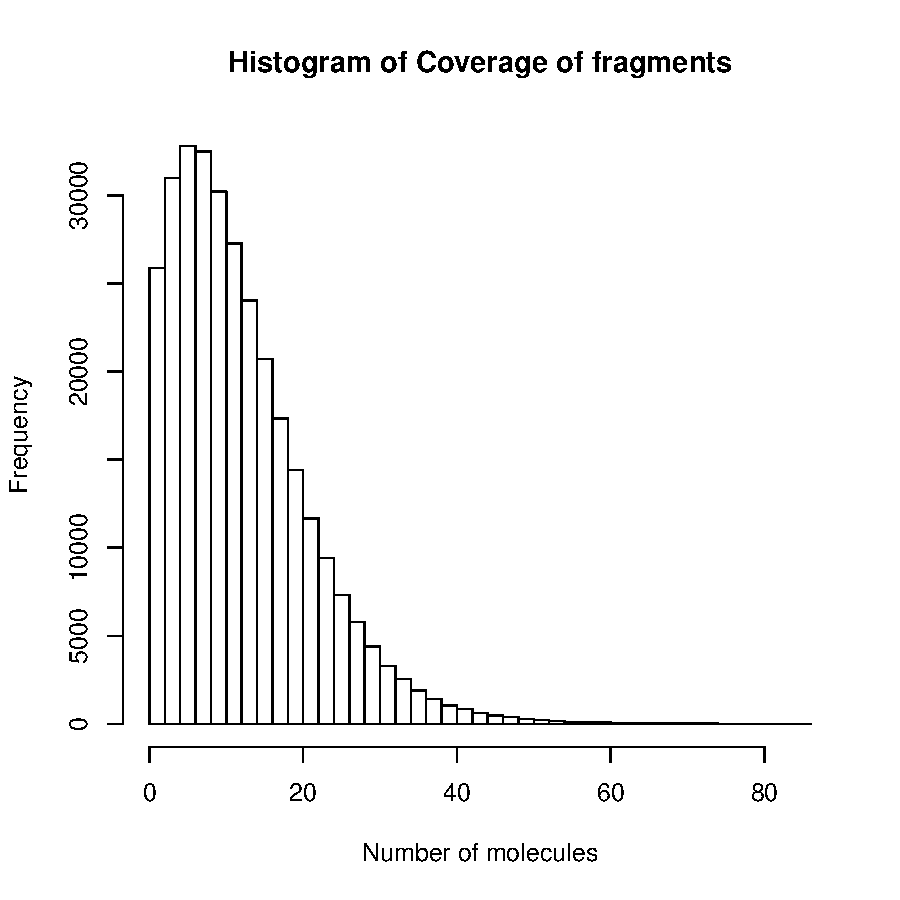
\includegraphics{GCvsIntensity_Report1-003}
% \caption{Some exploratory plots of the Data} % title of Table
% \label{fig:Fig1}
\end{figure}

When the variable $intensity\_mean$ is regressed with $fractionGC\_mean$ (or $GC-content$), the coefficient is quite significant (with p-value $<e^{-16}$, but the overall $R^2$ is only $2.5\%$. Similary, $intensity\_sd$ also has a significant relationship with $GC-content$, but the model $R^2$ is quite poor. There is evidence of a positive relationship between fluoroscence intensity and GC-content, however, more in-depth analysis is required. 

\section{Step 2: Modeling intensity and GC-content}
Prof. Schwartz recommended that we analyze only those fragments that have at least 40 coverage. Hence, the following analysis is conducted on the original dataset trimmmed down to only those fragments that have at least 40 molecules aligned to the same genomic location. This trimmed dataset has $35,040$ molecules and $4,513$ groups. The following models were fit:
\begin{enumerate}
\item
$Model1:\\ Y = log(intensity) \\ X = gc\_content$
\item
$Model2:\\ Y = log(intensity) \\ X = gc\_content + numFrags$ \\
numFrags is a measure of the number of fragments the molecule was divided into.
\item
$Model3:\\ Y = log(intensity) \\ X = gc\_content + numFrags + as.factor(groupID)$ \\
This model is to study how much of variability the channels on the surface contribute to that of the observed fluoroscence intensity.
\item
$Model4:\\ Y = log(intensity) \\ X = gc\_content + numFrags + as.factor(groupID) + numPixels$ \\
numPixels is a measure of the length (or size) of the molecule. Higher the number of pixels, longer the molecule. 
\end{enumerate}

Below are the R-outputs of the above mentioned models, and their anovas.\\
\noindent
{\bf{\underline{Summary of Model 1}}}
\begin{Schunk}
\begin{Soutput}
Call:
lm(formula = log(intensityPerPixel) ~ fractionGC, data = Data)

Residuals:
    Min      1Q  Median      3Q     Max 
-3.5223 -0.0884 -0.0257  0.0515  2.6821 

Coefficients:
             Estimate Std. Error t value Pr(>|t|)    
(Intercept) 10.440891   0.002649 3941.40   <2e-16 ***
fractionGC   0.179266   0.005808   30.86   <2e-16 ***
---
Signif. codes:  0 ‘***’ 0.001 ‘**’ 0.01 ‘*’ 0.05 ‘.’ 0.1 ‘ ’ 1 

Residual standard error: 0.1507 on 172560 degrees of freedom
Multiple R-squared: 0.00549,	Adjusted R-squared: 0.005484 
F-statistic: 952.6 on 1 and 172560 DF,  p-value: < 2.2e-16 
\end{Soutput}
\end{Schunk}
\noindent
{\bf{\underline{Summary of Model 2:}}}
\begin{Schunk}
\begin{Soutput}
Call:
lm(formula = log(intensityPerPixel) ~ fractionGC + numFrags, 
    data = Data)

Residuals:
    Min      1Q  Median      3Q     Max 
-3.5280 -0.0882 -0.0250  0.0529  2.6872 

Coefficients:
              Estimate Std. Error t value Pr(>|t|)    
(Intercept)  1.046e+01  2.723e-03 3840.51   <2e-16 ***
fractionGC   1.872e-01  5.806e-03   32.23   <2e-16 ***
numFrags    -6.518e-04  2.606e-05  -25.01   <2e-16 ***
---
Signif. codes:  0 ‘***’ 0.001 ‘**’ 0.01 ‘*’ 0.05 ‘.’ 0.1 ‘ ’ 1 

Residual standard error: 0.1504 on 172559 degrees of freedom
Multiple R-squared: 0.009081,	Adjusted R-squared: 0.009069 
F-statistic: 790.7 on 2 and 172559 DF,  p-value: < 2.2e-16 
\end{Soutput}
\end{Schunk}
\noindent
{\bf{\underline{Anova between Model1 and Model2}}}
\begin{Schunk}
\begin{Soutput}
Analysis of Variance Table

Model 1: log(intensityPerPixel) ~ fractionGC
Model 2: log(intensityPerPixel) ~ fractionGC + numFrags
  Res.Df    RSS Df Sum of Sq      F    Pr(>F)    
1 172560 3919.4                                  
2 172559 3905.3  1    14.152 625.31 < 2.2e-16 ***
---
Signif. codes:  0 ‘***’ 0.001 ‘**’ 0.01 ‘*’ 0.05 ‘.’ 0.1 ‘ ’ 1 
\end{Soutput}
\end{Schunk}

\noindent
{\bf{\underline{Summary of Model 3}}}
\begin{Schunk}
\begin{Soutput}
                              Estimate   Std. Error    t value     Pr(>|t|)
(Intercept)               1.040696e+01 4.844281e-02 214.829720 0.000000e+00
fractionGC                1.661665e-01 3.999466e-03  41.547175 0.000000e+00
numFrags                  2.112847e-04 1.955842e-05  10.802747 3.410075e-27
as.factor(groupID)2327861 2.019527e-01 5.534304e-02   3.649108 2.632321e-04
\end{Soutput}
\begin{Soutput}
[1] "R-Squared of Model 3:"
\end{Soutput}
\begin{Soutput}
[1] 0.6005285
\end{Soutput}
\end{Schunk}

\noindent
{\bf{\underline{Anova between Model2 and Model3}}}
\begin{Schunk}
\begin{Soutput}
Analysis of Variance Table

Model 1: log(intensityPerPixel) ~ fractionGC + numFrags
Model 2: log(intensityPerPixel) ~ fractionGC + numFrags + as.factor(groupID)
  Res.Df    RSS   Df Sum of Sq      F    Pr(>F)    
1 172559 3905.3                                    
2 168047 1574.3 4512    2330.9 55.143 < 2.2e-16 ***
---
Signif. codes:  0 ‘***’ 0.001 ‘**’ 0.01 ‘*’ 0.05 ‘.’ 0.1 ‘ ’ 1 
\end{Soutput}
\end{Schunk}

\noindent
{\bf{\underline{Summary of Model 4}}}
\begin{Schunk}
\begin{Soutput}
                Estimate   Std. Error    t value    Pr(>|t|)
(Intercept) 1.040686e+01 4.844157e-02 214.833244 0.000000000
fractionGC  1.689447e-01 4.097489e-03  41.231277 0.000000000
numFrags    9.119976e-05 4.320786e-05   2.110721 0.034797741
numPixels   2.630645e-06 8.440152e-07   3.116822 0.001828429
\end{Soutput}
\begin{Soutput}
[1] "R-Squared of Model 4:"
\end{Soutput}
\begin{Soutput}
[1] 0.6005516
\end{Soutput}
\end{Schunk}

\noindent
{\bf{\underline{Anova between Model3 and Model4}}}
\begin{Schunk}
\begin{Soutput}
Analysis of Variance Table

Model 1: log(intensityPerPixel) ~ fractionGC + numFrags + as.factor(groupID)
Model 2: log(intensityPerPixel) ~ fractionGC + numFrags + numPixels + 
    as.factor(groupID)
  Res.Df    RSS Df Sum of Sq      F   Pr(>F)   
1 168047 1574.3                                
2 168046 1574.2  1  0.091006 9.7146 0.001828 **
---
Signif. codes:  0 ‘***’ 0.001 ‘**’ 0.01 ‘*’ 0.05 ‘.’ 0.1 ‘ ’ 1 
\end{Soutput}
\end{Schunk}

\noindent
{\bf{\underline{Conclusion}}}: Introducing the groups as factors seem to explain $60\%$ of the variability. Since there are more than $35,000$ molecules, we can only check the molecule level effect for a few 100 molecules at a time. Given that so much variability in the response is a result of experimental artifacts, do you think there is any value proceeding with this project? Interestingly, the relationship between fluoroscence intensity and gc\_content remains significant even after introducing the group level effects.

\end{document}
